% Copyright (C) 2012 The ESPResSo project
%  
% This file is part of ESPResSo.
%   
% ESPResSo is free software: you can redistribute it and/or modify it
% under the terms of the GNU General Public License as published by the
% Free Software Foundation, either version 3 of the License, or (at your
% option) any later version.
%  
% ESPResSo is distributed in the hope that it will be useful, but
% WITHOUT ANY WARRANTY; without even the implied warranty of
% MERCHANTABILITY or FITNESS FOR A PARTICULAR PURPOSE.  See the GNU
% General Public License for more details.
%  
% You should have received a copy of the GNU General Public License
% along with this program.  If not, see <http://www.gnu.org/licenses/>.
%
\newcommand{\taumax}{\tau_{\mathrm{max}}}
\newcommand{\taumin}{\tau_{\mathrm{min}}}

\chapter{Analysis in the core}
\label{chap:analysis-core}
\index{Analysis in the Core}

Analysis in the core is a new concept introduced in \es since version 3.1.
It was motivated by the fact, that sometimes it is desirable that the analysis
functions do more than just return a value to the scripting interface.
For some observables it is desirable to be sampled every few
integrations steps. In addition, it should be possible to pass the
observable values to other functions which compute history-dependent
quantitites, such as correlation functions.  
All this should be done without the need to interrupt
the integration by passing the control to the script level and back, which
produces a significant overhead when performed too often. 

Some observables in the core have their corresponding counterparts
in the TCL observables of the \verb!analyze! command
described in Chapter~\ref{chap:analysis}. 
However, only the core-observables can be used on the fly with the 
toolbox of the correlator and on the fly analysis of time series.
Similarly, some special cases of using the correlator have their redundant
counterparts in the analysis in Tcl (Chapter~\ref{chap:analysis}),
but the correlator provides a general and versatile toolbox which
can be used with any implemented core-observables.

\section{Observables}
\index{Observables}

\newescommand{observable}

\subsection{Introduction}
The first step of the core analysis is to tell \es to create an observable.
That means just allocating the corresponding memory, assigning a function 
to compute the observable value and an \var{id} which will be used to refer 
to the observable. 
In addition to the possibility to  print the observable value 
(return the observable value to the script interface), 
the \var{id} of a core-observable can be passed to another analysis function. 
The observable value is computed from the current state of the system
at the moment when it is needed, \ie when requested explicitly by the 
user calling the \verb!observable print! function or when requested
automatically by some other analysis function.

Not all observables are implemented in parallel. When performing a parallel
computation, too frequent updates to observables which are not implemented
in parallel may produce a significant slowdown.

\subsection{Creating an observable}
To create a new observable, use
\begin{essyntax}
  observable new \var{name} \opt{\var{parameters+}}
\end{essyntax}
  
Upon this call, \es allocates the necessary amount of memory and returns 
an integer \var{id} which will be used later to refer to the observable. 
The parameter \var{name} and further arguments have to correspond to one of the
observables described below.

\subsubsection{Available observables}
Currently the following observables are implemented.
Particle specifications (see section~\ref{sec:PartSpec} below)
define a group of particles, from which the observable should be calculated. 
They are generic to all observables and are described after the list of observables.

\todo{Missing descriptions of parameters of several observables}
  \begin{itemize}
    \item \lit{particle_positions} \var{particle\_specifications}\\
          Positions of the particles, in the format 
          $x_1,\ y_1,\ z_1,\ x_2,\ y_2,\ z_2,\ \dots\ x_n,\ y_n,\ z_n$. The particles 
          are ordered ascending according to their ids.
    \item \lit{particle_velocities} \var{particle\_specifications}\\
          Velocities of the particles, in the format\\ 
          $v^x_1,\ v^y_1,\ v^z_1,\ v^x_2,\ v^y_2,\ v^z_2,\ 
          \dots\ v^x_n,\ v^y_n,\ v^z_n$. 
          The particles are ordered ascending according to their ids.
    \item \lit{com_velocity} \var{particle\_specifications}\\
          Velocity of the centre of mass
    \item \lit{com_position} \var{particle\_specifications}\\
          Position of the centre of mass
    \item \lit{stress_tensor} \\
          The stress tensor. It only works with all particles. 
          It is returned as a 9-dimensional array:\\
          $ \{\ \sigma_{xx},\ \sigma_{xy},\ \sigma_{xz},\ \sigma_{yx},\ \sigma_{yy},\
          \sigma_{yz},\ \sigma_{zx},\ \sigma_{zy},\ \sigma_{zz}\ \} $
    \item \lit{stress_tensor_acf_obs} \\
          The observable for computation of the Stress tensor autocorrelation function. 
          Same as stress tensor, it only works with all particles.
          It is returned as a 6-dimensional array:\\
          $ \{\ \sigma_{xy},\ \sigma_{yz},\ \sigma_{zx},\ 
          ( \sigma_{xx} - \sigma_{yy}),\ 
          ( \sigma_{xx} - \sigma_{zz}),\ 
          ( \sigma_{yy} - \sigma_{zz})\  
          \} $ \\
          where $\sigma_{ij}$ are the components of the stress tensor.
    \item \lit{particle_currents} \var{particle\_specifications}\\
    \item \lit{currents} \var{particle\_specifications}\\
    \item \lit{dipole_moment} \var{particle\_specifications}\\
    \item \lit{structure_factor} \var{particle\_specifications}\\
    \item \lit{interacts_with} \var{particle\_specifications\_1} \var{particle\_specifications\_2} \var{cutoff} \\
          For each particle belonging to \var{particle\_specifications\_1} 
          the observable is unity if a neighbour of a type from 
          \var{particle\_specifications\_2} is found within the distance 
          defined by the \var{cutoff}. If no such neighbour is found, the 
          observable is zero. The observable has as one dimension per each 
          particle of \var{particle\_specifications\_1}
    \item \lit{nearest_neighbour_conditional} \\
          For each particle belonging to \var{type\_list\_1} return the particle id
	  of the nearest neighbour which has a particle type from \var{type\_list\_2}. 
	  If no such neighbour is found within the \var{cutoff}, it returns -1. 
	  The observable has 2 dimensions per particle of \var{type\_list\_1}. First
	  value is the neighbour id, the second one is the condition. Condition is
	  incremented when the particle state changes from \emph{no partners}
	  to \emph{some partner} or vice versa. In addition, in the former case
	  also the sign is changed.
          
    \item \lit{density_profile}
    \item \lit{lb_velocity_profile}
    \item \lit{radial_density_profile}
    \item \lit{radial_flux_density_profile}
    \item \lit{flux_density_profile}
    \item \lit{lb_radial_velocity_profile}
    \item \lit{textfile \var{textfilename} \opt{\var{column\_1} \dots \var{column\_n} }}
      This option allows to read data from an arbitrary text file, organized in columns.
      The name of the textfile is 
      \todo{Texfile input observable not fully supported yet!}
    \item \lit{tclinput \var{dimQ} } TCL input of length  \var{dimQ} is used as ``observable''. 
      \todo{Tcl input observable not fully supported yet!}
  \end{itemize}

\subsection{Printing an observable}
\begin{essyntax}
observable \var{id} print \opt{formatted}
\end{essyntax}
Prints the value of the observable with a given $id$. If the observable
refers to the current state of the system, its value is updated before printing.
\todo{Formatted printing is not fully supported yet.}

\subsection{Passing an observable to an analysis function}
Currently the only analysis function which uses the core observables
is the correlator (section~\ref{sec:Correlations}).

\subsection{Deleting an observable to an analysis function}
\begin{essyntax}
observable \var{id} delete
\end{essyntax}
Deletes the observable, \ie frees the allocated memory
and makes the $id$ free for a new observable.
\todo{Does not work yet}


\subsection{Particle specifications}
\label{sec:PartSpec}
You can specify from which particles the observable should be computed in one of 
the following ways. In all cases, particle specifications refer to the current
state of espresso. Any later changes to particles (additions, deletions, changes
of types) will not be automatically reflected in the observable.
  \begin{itemize}
    \item \lit{all} \\
          Requests observable calculation based on all particles in the system.
    \item \lit{types} \var{ type\_list } \\
          Restricts observable calculation to a given particle type(s). The type
	  list is a tcl list of existing particle types.
    \item \lit{id} \var{ id\_list } \\
          Restricts observable calculation to a given list of particle id(s). The id 
	  list is a tcl list of existing particle ids.
% The following two particle specifications have not been implemented yet
%    \item \lit{blocks} \var{ m } \\
%          From an $n$-dimensional observable craeates an $n/m$-dimensional one by 
%	  averaging over $m$ neighbouring entries in the data array.
%      \todo{Not fully supported yet!}
%    \item \lit{strides} \var{ m } \\
%          From an $n$-dimensional observable craeates an $n/m$-dimensional one by 
%	  averaging over entries which are separated by $m$ in the data array.
%      \todo{Not fully supported yet!}
  \end{itemize}



\section{Correlations}
\index{Correlations}
\label{sec:Correlations}

\subsection{Introduction}
Time correlation functions are ubiquitous in statistical mechanics and molecular
simulations when dynamical properties of many-body systems are concerned.
A prominent example is the velocity autocorrelation function,  
$ \left< \mathbf{v}(t) \cdot \mathbf{v}(t+\tau) \right> $ 
which is used in the Green-Kubo relations.
In general, time correlation functions are of the form
\begin{equation}
C(\tau) = \left<A\left(t\right) \otimes B\left(t+\tau\right)\right>\,,
\label{eq:corr.def}
\end{equation}
where $t$ is time, $\tau$ is the lag time (time difference) between 
the measurements of (vector) observables $A$ and $B$, and $\otimes$ is an
operator which produces the vector quantity $C$ from $A$ and $B$. 
The ensemble average $\left< \cdot \right>$ is taken over all time origins~$t$. 
Correlation functions describing dynamics of large and complex molecules 
such as polymers span many orders of magnitude, ranging from MD time step
up to the total simulation time. 

\es uses a fast correlation algorithm (see section~\ref{sec:multipleTau})
which enables efficient computation of correlation functions spanning
many orders of magnitude in the lag time. 

The generic correlation interface of \es may process either observables
defined in the kernel, or data which it reads from an external file
or values entered through the scripting interface. 
\todo{Processing data from TCL input or from input files is not
  fully supported yet.}
Thus, apart from
data processing on the fly, it can also be used as an efficient correlator
for stored data. In all cases it produces a matrix of 
$n+2$ columns. The first two columns are the values of lag times $\tau$ and 
the number of samples taken for a particular value of $\tau$. The
remaining ones are the elements of the $n$-dimensional vector $C(\tau)$.

The \lit{uwerr} command for computing averages and error estimates 
of a time series of observables relies on estimates of autocorrelation
functions and the respective autocorrelation times.
The correlator provides the same functionality as a by-product of comupting
the correlation function (see section~\ref{ssec:CorrError}.

An example of the usage of observables and correlations is provided 
in the script \lit{correlation.tcl} in the samples directory.


\subsection{Creating a correlation}
\newescommand{correlation}

Correlation first has to be defined by saying which observables 
are to be correlated, what should be the correlation operation, sampling
frequency, etc. When a correlation is defined, its id is returned which is
used further to do other operations with the correlation.
The correlation can be either updated automatically on the fly without
direct user intervention, or by an explicit user call for an update.

\begin{essyntax}
correlation new obs1 \var{id1} \opt{obs2 \var{id2}} corr_operation \var{operation} dt \var{dt} tau_max \var{tau\_max} \opt{tau_lin \var{tau\_lin}} \opt{compress1 \var{name} \opt{compress2 \var{name}} }
\end{essyntax}

Defines a new correlation and returns an integer
\var{id} which has been assigned to it. 
Its further arguments are described below.

\begin{arguments}
\item \lit{obs1} and \lit{obs2} \\ 
  are ids of the observables A and B that are to correlated. The ids have to refer to existing 
  observables which have been previously defined by the \lit{observable} command.
  Some observables are already implemented, and others can be easily added. This can be done
  with very limited \es{} knowledge just by following the implementations that are already
  in. If \lit{obs2} is omitted, autocorrelation of \lit{obs1} is calculated by default.
\item \lit{corr_operation} \\
  The operation that is performed on $A(t)$ and $B(t+\tau)$ to obtain $C(\tau)$. 
  The following operations are currently is available:
  \begin{itemize}
    \item \lit{scalar_product} \\
    Scalar product of $A$ and $B$, \ie $C=\sum\limits_{i} A_i B_i$
    \item \lit{componentwise_product} \\
    Comnponentwise product of $A$ and $B$, \ie $C_i = A_i B_i$
    \item \lit{square_distance_componentwise} \\
    Each component of the correlation vector is the square of the difference between the 
    corresponding components of the observables, \ie $C_i = (A_i-B_i)^2$. 
    Example: when $A$ is \lit{particle_positions}, it produces the mean square displacement
    (for each componnent separately).
    \item \lit{complex_conjugate_product}
    %\item List them here! \todo{write the list}
  \end{itemize}
\item \lit{dt} \\
  The time interval of sampling data points. When autoupdate is used, \var{dt} has
  to be a multiple of timestep. It is also used to produce time axis in real units.
  \textit{Warning: if \var{dt} is close to the timestep, autoupdate is strongly recommended.
  Otherwise cpu time is wasted on passing the control between the script and kernel.}
\item \lit{tau_max} \\
  This is the maximum value of $\tau$ for which the correlation should be computed.
  \textit{Warning: Unless you are using the multiple tau correlator, choosing \var{tau\_max}
  of more than 100\var{dt} will result in a huge computational overhead.
  In a multiple tau correlator with reasonable parameters, 
  \var{tau\_max} can span the entire simulation without
  too much additional cpu time.}
\item \lit{tau_lin} \\
  The number of datapoints for which the results are linearly spaced
  in tau.  This is a parameter of the multiple tau correlator. If you
  want to use it, make sure that you know how it works. By default, it
  is set equal to \var{tau\_max} which results in the trivial linear
  correlator. By setting \var{tau\_lin} < \var{tau\_max} the multiple
  tau correlator is switched on. In many cases, \var{tau\_lin}=16 is a
  good choice but this may strongly depend on the observables you are
  correlating.  For more information, we recommend to read
  Ref.~\cite{ramirez10a} or to perform your own tests.
\item \lit{compress1} and \lit{compress2} \\
  Are functions used to compress the data when going to the next level
  of the multiple tau correlator. Different compression functions for
  different observables can be specified if desired, otherwise the
  same function is used for both.  Default is \lit{discard} which
  takes one of the observable values and discards the other one. This
  is safe for all observables but produces poor statistics in the
  tail. For some observables, \lit{linear} compression can be used
  which makes an average of two neighbouring values but produces
  systematic errors.  Depending on the observable, the systematic
  error can be anything between harmless and disastrous. For more
  information, we recommend to read Ref.~\cite{ramirez10a} or to
  perform your own tests.
\end{arguments}

\subsection{Inquiring about already existing correlations}
\begin{essyntax}
\variant{1} correlation 
\variant{2} correlation n_corr
\end{essyntax}

Variant \variant{1} returns a tcl list of the defined correlations
including their parameters.  \todo{Maybe not all parameters are
  printed.}  

Variant \variant{2} returns the number of currently
defined correlations.  
  
\subsection{Collecting time series data for the correlation}

\begin{essyntax}
\variant{1} correlation \var{id} autoupdate \{ start | stop\} 
\variant{2} correlation \var{id} update 
\variant{3} correlation \var{id} finalize
\end{essyntax}

Variant \variant{1} is the recommended way of updating the correlations.
By specifying \lit{start} or \lit{stop} it starts or stops automatically
updating the correlation estimates. The automatic updates are done
within the integration loop without furhter user interventin.
The update frequency is adjusted based based on the value of \var{dt} 
provided when defining the correlation.  

Variant \variant{2} is an explicit call for an instantaneous 
update of the correlation estimates, using the current system
state. It is only possible to use \variant{2} if the correlation
is not being autoupdated. However, it is possible to use it
after autoupdate has been stopped. When updating by an explicit
call, \es does not check if the lag time between two updates
corresponds the value of \var{dt} specified when creating the 
correlation.

Variant \variant{3} correlates all data from history which are left in
the buffers. Once this has been done, the history is lost and no
further updates are possible. 
When a new observable value is passed to a correlation,
level 0 of the compression buffers of the multiple tau
correlator (see section~\ref{sec:multipleTau} for details) 
is updated immediately. Higher levels are
updated only when the lower level buffers are filled and
there is a need to push some values one level up. When the
updating is stopped, a number of observable values have not
reached the higher level, especially when \var{tau_max} 
is comparable to the total simulation time
and if there are many compression levels. In such case,
variant \variant{3} is very useful. If \var{tau\_max} 
is much shorter, it does not have a big effect.


\subsection{Printing out the correlation and related quantities}
\label{ssec:CorrError}
\begin{essyntax}
\variant{1} correlation \var{id} write_to_file \var{filname}
\variant{2} correlation \var{id} print 
\variant{3a} correlation \var{id} print \opt{ average1 | variance1 | correlation_time } 
\variant{3b} correlation \var{id} print \opt{ avarage_errorbars }
\end{essyntax}

Variant \variant{1} writes the current status of the correlation
estimate to the specified filename. If the file exists, its contents will
be owerwritten.

\minisec{Output format} 
The output looks as follows:
\begin{code}
tau1 n_samples C1 C2 ... Cn
tau2 n_samples C1 C2 ... Cn
\end{code}
Where each line corresponds to a given value of \lit{tau}, \lit{n_samples} is the number
of samples which contributed to the correlation at this level and $C_i$ are the individual
components of the correlation.

Variant \variant{2} returns the current status of the correlation
estimate as a Tcl variable. 
\minisec{Output format} 
The output looks as follows:
\begin{code}
{ tau1 n_samples C1 C2 ... Cn }
{ tau2 n_samples C1 C2 ... Cn }
\end{code}

Variants \variant{3a} and \variant{3b} return the corresponding
estimate of the statistical property as a Tcl variable.             \\
\lit{average1} prints the average of observable1.                   \\
\lit{variance1} prints the variance of observable1.                 \\
\lit{correlation_time} prints the estimate of the correlation time. \\
\lit{average_errorbars} prints the estimate of the error of the average based
on the method according to~\cite{wolff04a} (same as 
used by the \lit{uwerr} comamnd). 


\subsection{The correlation algorithm: multiple tau correlator}
\label{sec:multipleTau}
\index{Multiple tau correlator}

Here we briefly describe the multiple tau correlator which is implemented in \es.
For a more detailed description and discussion of its behaviour with respect to
statistical and systematic errores, please read the cited literature.
This type of correlator has been in use for years in the analysis of
dynamic light scattering~\cite{schatzel88a}. About a decade later it found its way
to the Fluorescence Correlation Spectroscopy (FCS)~\cite{magatti01a}.
The book of Frenkel and Smit~\cite{frenkel02b} describes its application
for the special case of the velocity autocorrelation function.

\begin{figure}[ht]
\begin{center} 
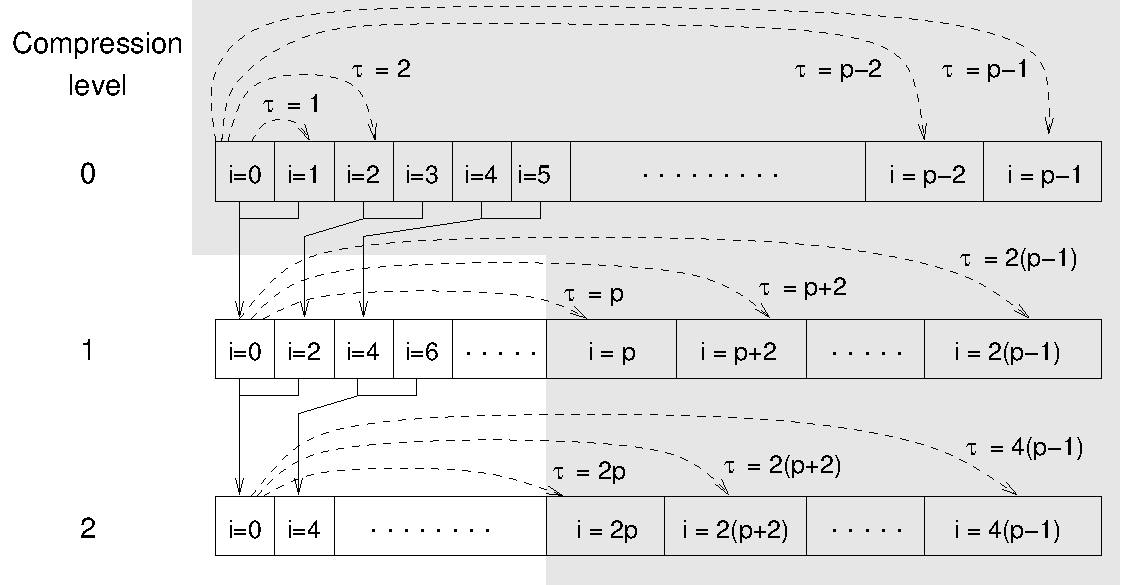
\includegraphics[width=0.9\textwidth]{figures/correlator_scheme}
\end{center} 
\caption{Schematic representation of buffers in the correlator.}
\label{fig:dataSet}
\end{figure}

Let us consider a set of $N$ observable values as schematically shown
in Figures~\ref{fig:dataSet}, where a value of index $i$ was measured
in time $i\delta t$. We are interested in computing the correlation 
function according to Equation~\ref{eq:CtauDef} for a range lag times
$\tau = (i-j)\delta t$ between the measurements $i$ and $j$.
To simplify the notation, we further drop $\delta t$
when refering to observables and lag times. 

The trivial implementation takes all possible pairs of values
corresponding to lag times $\tau \in [\taumin:\taumax]$. 
Without loss of generality, let us further consider $\taumin=0$.
The computational effort for such an algorithm scales
as ${\cal O} \bigl(\taumax^2\bigr)$.
As a rule of thumb, this is feasible if $\taumax < 10^3$.
The multiple tau correlator provides a solution to compute the
correlation functions for arbitrary range of the lag times by
coarse-graining the high $\tau$ values. It applies the naive algorithm
to a relatively small range of lag times $\tau \in [0:p-1]$. This we refer
to as compression level 0. To compute the correlations for lag times
$\tau \in [p:2(p-1)]$, the original data are first coarse-grained, so
that $m$ values of the original data are compressed to produce a single
data point in the higher compression level. Thus the lag time between
the neighbouring values in the higher compression level increases
by a factor of $m$, while the number of stored values decreases by
the same factor and the number of correlation operations at this level
reduces by a factor of $m^2$. Correlations for lag times 
$\tau \in [2p:4(p-1)]$ are computed at compression level 2, which is created
in an analogous manner from level 1. This can continue hierarchically
up to an arbitrary level for which enough data is available. Due to the
hierarchical reduction of the data, the algorithm scales as 
${\cal O} \bigl( p^2 \log(\taumax) \bigr)$. Thus an additional order
of magnitude in $\taumax$ costs just a constant extra effort.

The speedup is gained at the expense of statistical accuracy.
The loss of accuracy occurs at the compression step.
In principle one can use any value of $m$ and $p$ to tune the algorithm
performance. However, it turns out that using a high $m$ dilutes the
data at high $\tau$. Therefore $m=2$ is hardcoded in the \es correlator
and cannot be modified by user. The value of $p$ remains an adjustable
parameter which can be modified by user by setting \lit{tau_lin}
when defining a correlation. In genral, one should choose $p \gg m$
to avoid loss of statistical accuracy. Choosing $p=16$ seems to be
safe but it may depend on the properties of the analyzed
corerlation functions. A detailed analysis has been performed
in Ref.~\cite{ramirez10a}.

The choice of the compression function also influences the statistical
accuracy and can even lead to systematic errors. The default compression 
function is \lit{discard2} which discards the second fo the compressed 
values and pushes the first one to the higher level. This is robust and 
can be applied universally to any combination of observables and
correlation operation. On the other hand, it reduces the
statistical accuracy as the compression level increases.
In many cases, the \lit{average} compression operation
can be applied, which averages the two neighbouring values
and the average then enters the higher level, preserving
almost the full statistical accuracy of the original data. 
In general, if averaging can be safely used or not, depends on the 
properties of the difference
\begin{equation} 
\frac{1}{2} (A_i \otimes B_{i+p} + A_{i+1} \otimes B_{i+p+1} ) - 
\frac{1}{2} (A_i + A_{i+1} ) \otimes \frac{1}{2} (B_{i+p} +  B_{i+p+1})
\label{eq:difference}
\end{equation} 
For example in the case of velocity autocorrelation function, the
above-mentioned difference has a small value and a random sign, \ie\ 
different contributions cancel each other. On the other hand, in the
of the case of mean square displacmenent the difference is always positive,
resulting in a non-negligible systematic error. A more general
discussion is presented in Ref.~\cite{ramirez10a}.
